\documentclass[10pt,a4paper]{article}
\usepackage[margin=1.55cm]{geometry}
\usepackage[T1]{fontenc}
\usepackage[utf8]{inputenc}
\usepackage{lmodern}
\usepackage{booktabs}
\usepackage{graphicx}
\usepackage{xcolor}
\usepackage{hyperref}
\usepackage{enumitem}
\usepackage{amsmath}
\usepackage{amssymb}
\usepackage{titlesec}
\usepackage{fancyhdr}

\definecolor{navy}{HTML}{004E7C}
\definecolor{slate}{HTML}{4A5568}
\definecolor{accent}{HTML}{D55E00}

\hypersetup{colorlinks=true, linkcolor=navy, urlcolor=navy}
\titleformat{\section}{\large\bfseries\color{navy}}{}{0em}{}[\titlerule]
\titlespacing*{\section}{0pt}{7pt}{4pt}
\setlist[itemize]{noitemsep, topsep=2pt, leftmargin=1.4em}

\pagestyle{fancy}
\fancyhf{}
\lhead{\small\color{slate} Fundamentals of Machine Learning (UAB) --- Follow-up \#2 Review Brief (Dec 11)}
\rhead{\small\color{slate} Project Team 05}
\cfoot{\small\thepage}

\begin{document}

\begin{center}
  {\LARGE\bfseries\color{navy} Follow-up \#2 Deliverable: Model, Ablation \& iNterpret}\\[4pt]
  {\large Temporal Benchmark, 7-Subset Factor Group Ablation, ``What-If'' Studies \& Irreducible Error Appraisal}\\[5pt]
  {\small\color{slate} \textbf{Team 05:} Marc Font Hostalet, David Redrejo P\'erez, Elias Barreiro Pena \quad|\quad \textbf{Notebook:} \texttt{notebooks/02\_followup2\_model\_interpret.ipynb}}
\end{center}
\vspace{-4pt}

\section{1. Temporal Benchmark Results (CV 2017--2021 $\rightarrow$ Held-Out Test 2022--2024, $n=1{,}359$)}
\begin{table}[h!]
  \centering
  \footnotesize
  \setlength{\tabcolsep}{4.5pt}
  \begin{tabular}{llccccccc}
    \toprule
    \textbf{Model} & \textbf{Family} & \textbf{CV AUC} & \textbf{CV Acc} & \textbf{Test AUC} & \textbf{Test Acc} & \textbf{Test F1} & \textbf{Log-Loss} & \textbf{McNemar $p$} \\
    \midrule
    Baseline: \texttt{grid <= 10} (Scrubbed) & Baseline & 0.7520 & 75.20\% & 0.7712 & 77.12\% & 0.7708 & --- & \textit{(ref)} \\
    Baseline: Grid-Only Logistic & Baseline & 0.8186 & 75.20\% & 0.8316 & 77.12\% & 0.7708 & 0.5077 & --- \\
    \midrule
    \textbf{Logistic Regression (L2, $C=0.1$)} & Linear & 0.8387 & 76.67\% & 0.8708 & \textbf{80.43\%} & 0.7997 & 0.4522 & \textbf{0.0012} \\
    \textbf{Logistic Regression (L1, $C=0.01$)} & Linear & \textbf{0.8401} & \textbf{76.90\%} & 0.8728 & 79.84\% & 0.7964 & 0.4579 & \textbf{0.0087} \\
    \textbf{Linear SVM ($C=0.001$, Platt)} & Linear & 0.8376 & 76.23\% & 0.8717 & 79.76\% & 0.7943 & \textbf{0.4504} & \textbf{0.0061} \\
    Gaussian Naive Bayes & Probabilistic & 0.8323 & 76.39\% & 0.8609 & 80.28\% & 0.8027 & 1.5255 & 0.0017 \\
    k-Nearest Neighbors ($k=75$) & Instance & 0.8290 & 75.17\% & 0.8671 & 80.06\% & 0.8018 & 0.4613 & 0.0012 \\
    RBF Kernel SVM & Kernel & 0.8365 & 75.94\% & 0.8686 & 80.13\% & 0.8038 & 0.4524 & $<$0.0001 \\
    Decision Tree (Entropy, $d=4$) & Tree & 0.8201 & 74.65\% & 0.8554 & 78.59\% & 0.7846 & 0.4764 & 0.2475 \\
    Random Forest & Ensemble & \textbf{0.8401} & 76.19\% & \textbf{0.8734} & 79.91\% & 0.8020 & 0.4531 & \textbf{0.0062} \\
    Gradient Boosting & Ensemble & 0.8393 & 76.10\% & 0.8720 & \textbf{81.16\%} & \textbf{0.8153} & 0.4534 & \textbf{$<$0.0001} \\
    \bottomrule
  \end{tabular}
  \vspace{-4pt}
  \caption{\small All ML models tuned strictly on 5-fold expanding-window seasonal CV (2017--2021). L1 Logistic wins CV, matches Random Forest on Test (McNemar $p=1.000$, $\Delta\text{AUC}=-0.0006$), and Linear SVM achieves the lowest Test Log-Loss (0.4504).}
\end{table}

\begin{figure}[h!]
  \centering
  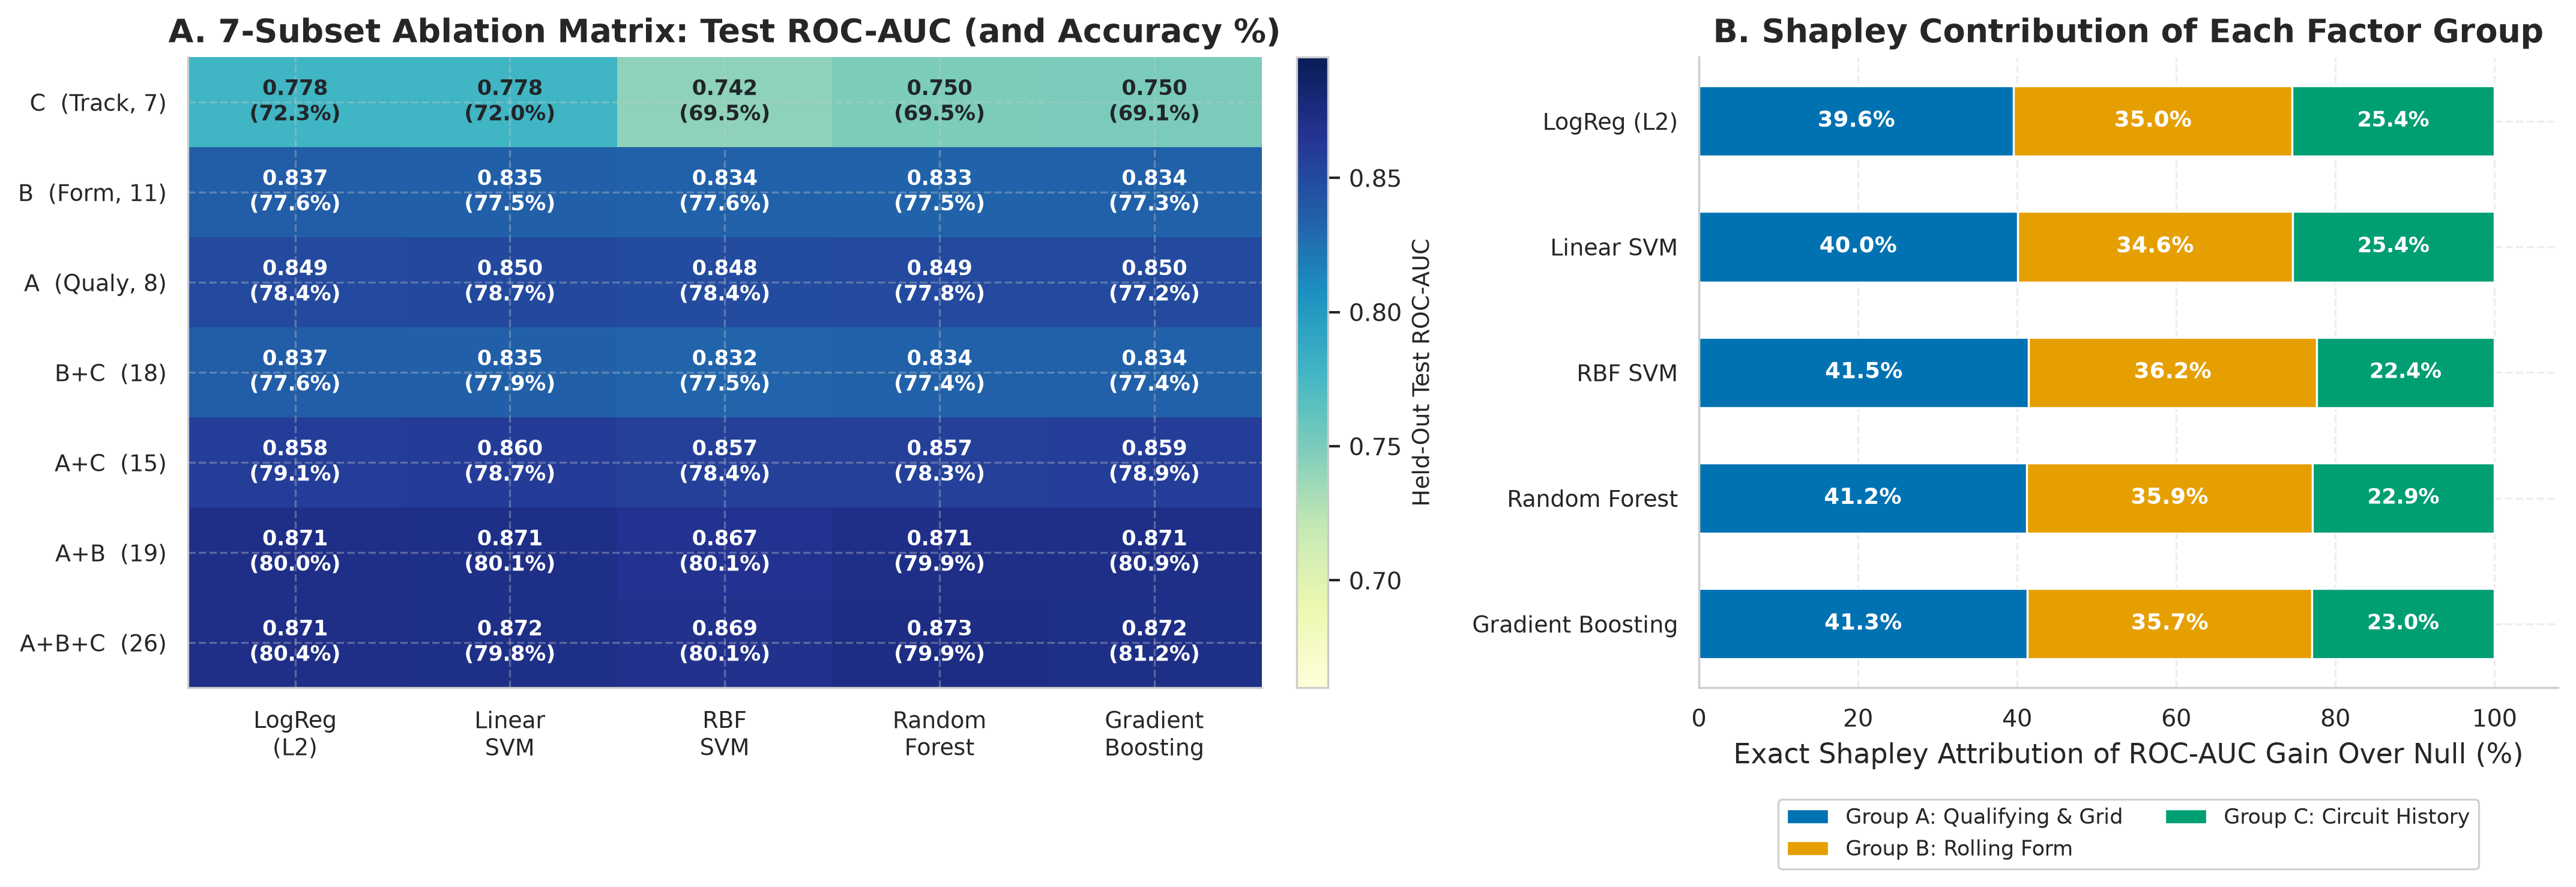
\includegraphics[width=0.98\textwidth]{../figures/followup2/fig08_ablation_7subsets_and_shapley.png}
  \vspace{-6pt}
  \caption{\small Centerpiece 7-subset ablation matrix across 5 model families (left) and exact 3-player Shapley attributions (right). Adding Group B to A raises Test ROC-AUC by $+0.019$ to $+0.022$ universally, while adding Group C to A+B yields $-0.0002$ to $+0.0025$.}
\end{figure}

\begin{itemize}
  \item \textbf{H1 Confirmed (Factor Hierarchy):} Qualifying (A) + Rolling Form (B) achieve virtually full performance (LogReg L2: 0.8710 AUC vs 0.8708 for A+B+C). Crucially, CV-optimal \textbf{L1 Lasso ($C=0.01$)} automatically zeroes out \textbf{all 7/7 Group C features}, retaining 4 Group A and 6 Group B features! Standalone C reaches $\sim$0.75--0.78 AUC only as a lagged proxy for persistent team quality.
  \item \textbf{H2 Confirmed with Nuance:} Regularized linear models statistically tie Random Forest (McNemar $p=1.000$) and lead in calibration (Linear SVM Log-Loss 0.4504, Brier 0.1428), whereas Gaussian NB suffers severe miscalibration (Log-Loss 1.5255) due to feature collinearity. Gradient Boosting gains $+0.74$ pp raw accuracy at $t=0.50$ without improving AUC or calibration.
\end{itemize}

\newpage

\section{2. ``What-If'' Regularization Paths, Decision Geometry \& Error Appraisal}

\begin{figure}[h!]
  \centering
  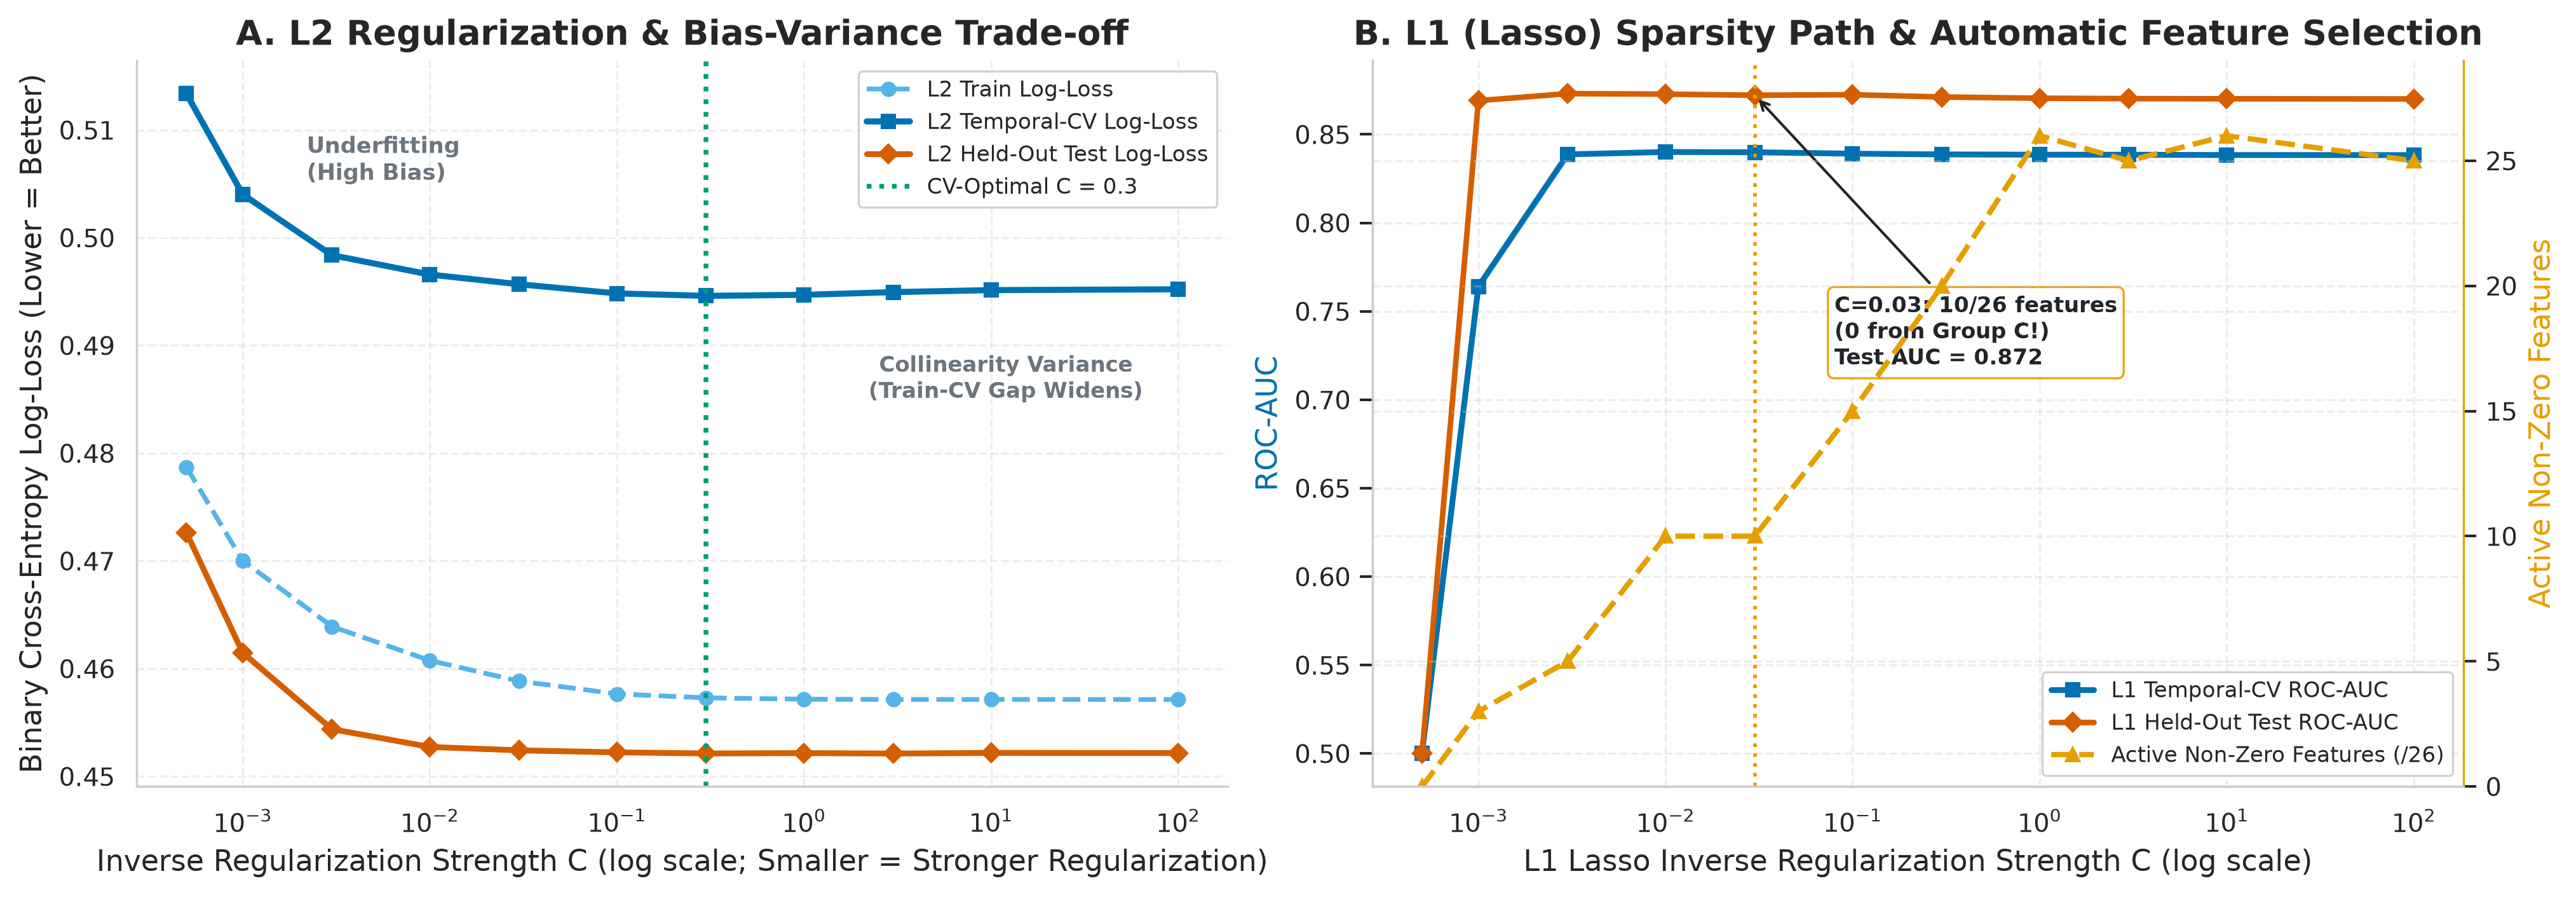
\includegraphics[width=0.98\textwidth]{../figures/followup2/fig09_regularization_and_bias_variance.png}
  \vspace{-6pt}
  \caption{\small L2 bias-variance curve across $C$ (left) and L1 sparsity path showing near-peak Test AUC (0.872) with only 10/26 active features---0 from Group C (right).}
\end{figure}

\begin{figure}[h!]
  \centering
  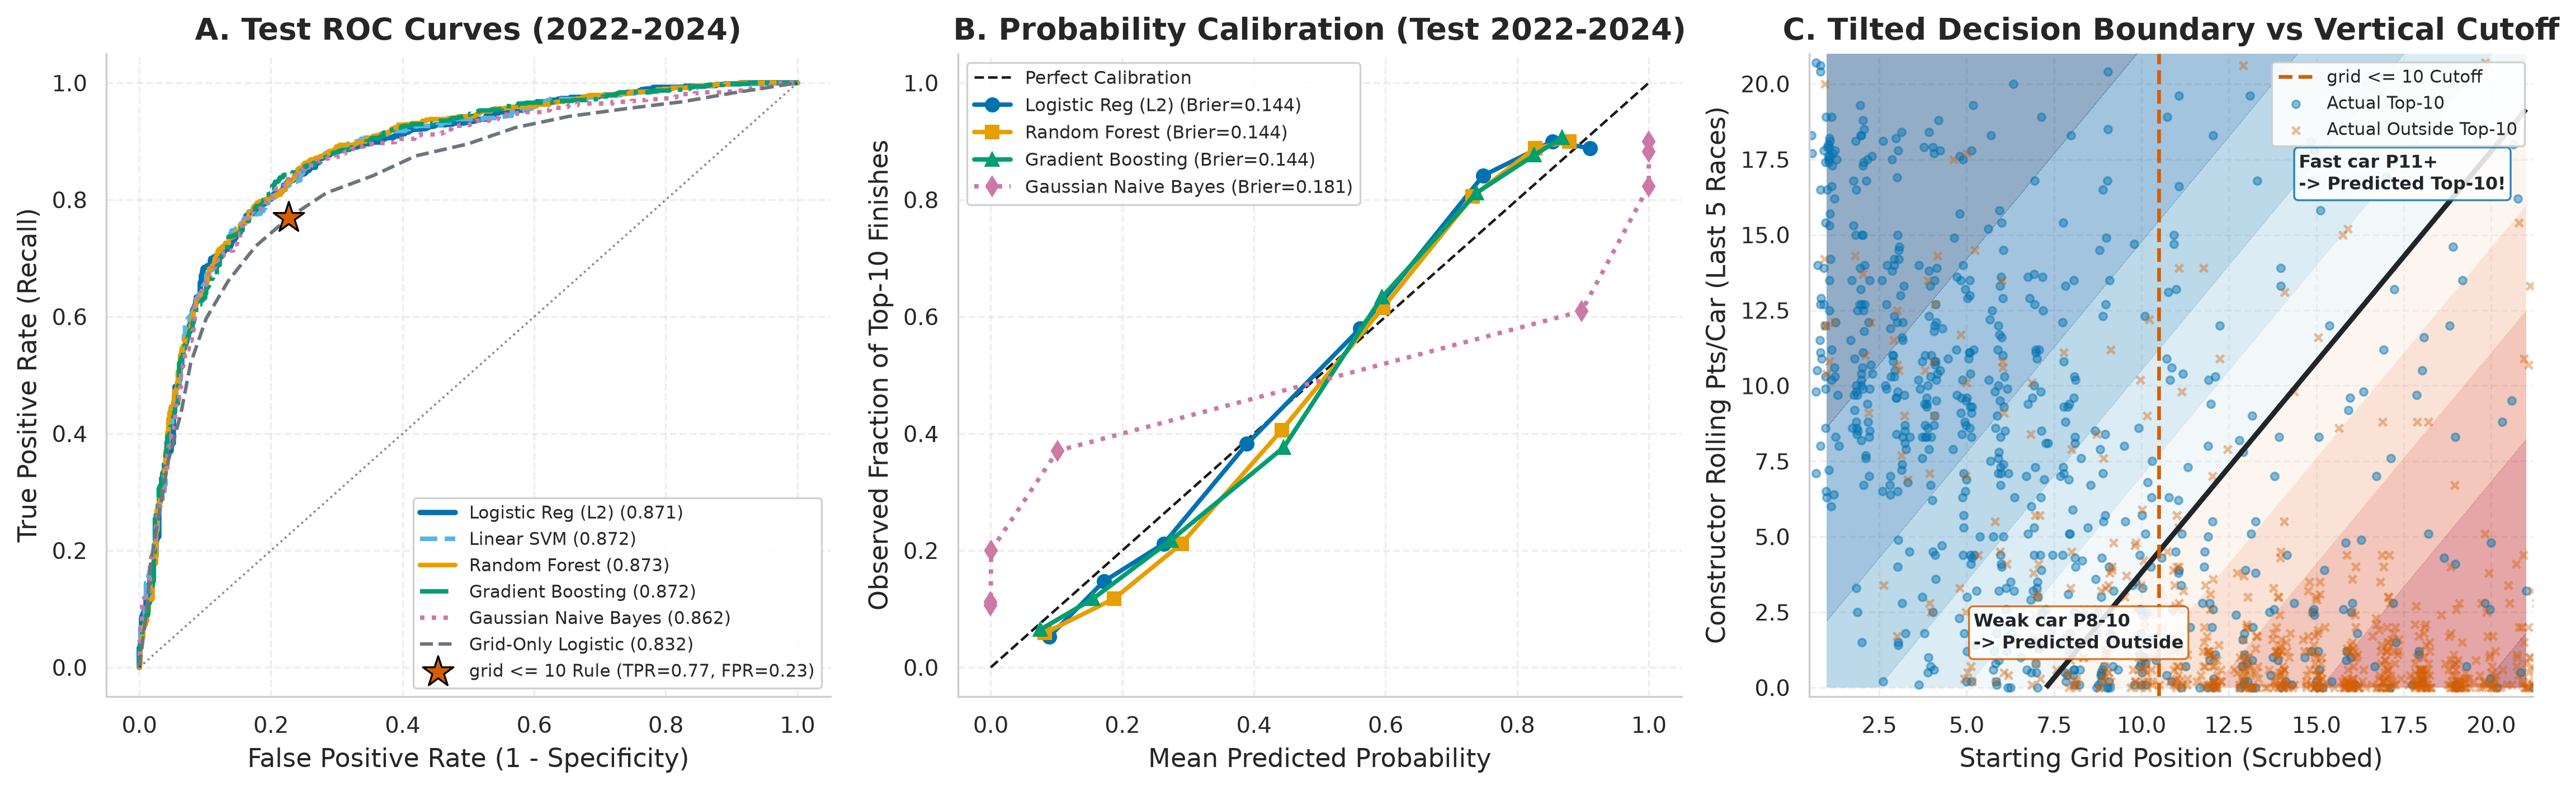
\includegraphics[width=0.98\textwidth]{../figures/followup2/fig11_roc_pr_calibration_and_boundary.png}
  \vspace{-6pt}
  \caption{\small ROC curves vs the \texttt{grid <= 10} operating star (left), reliability curves exposing Gaussian NB's collinearity miscalibration (center), and the tilted 2D linear boundary overturning the vertical \texttt{grid <= 10} cutoff for fast cars starting P11+ and slow cars starting P8--P10 (right).}
\end{figure}

\begin{figure}[h!]
  \centering
  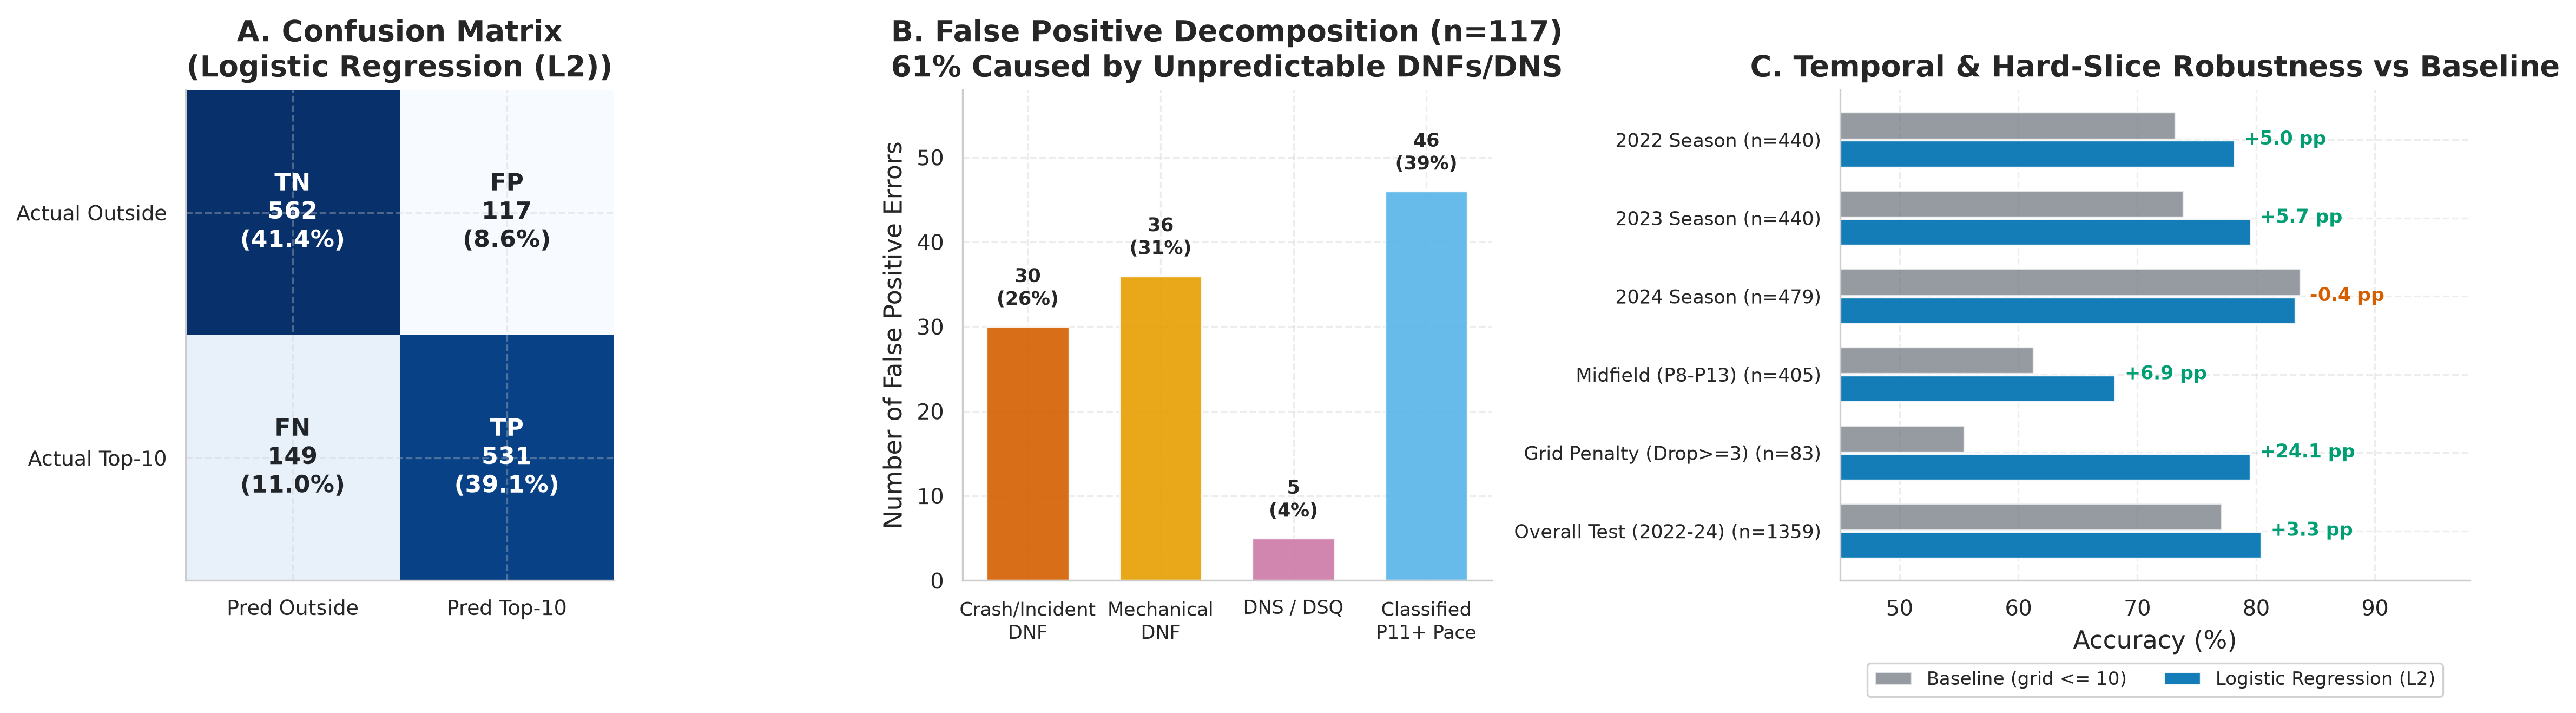
\includegraphics[width=0.98\textwidth]{../figures/followup2/fig12_error_analysis_and_regime_robustness.png}
  \vspace{-6pt}
  \caption{\small Confusion matrix (left), post-hoc False Positive error decomposition revealing 61\% stem from unpredictable DNFs/DNS (center), and slice gains showing \textbf{+24.1 pp} on Grid Penalty Drops and \textbf{+6.9 pp} in the P8--P13 Midfield Zone (right).}
\end{figure}

\section{3. Key ``What-If'' \& Critical Takeaways for Final Report}
\begin{itemize}
  \item \textbf{Rolling Window Sensitivity:} Longer smoothing ($W=10$: Test AUC 0.8751, Acc 80.35\%) slightly beats short windows ($W=3$: AUC 0.8702) by filtering out single-race DNF noise.
  \item \textbf{Canonical Team Lineages:} Improves rebranded constructor calibration on 2022--2024 (Log-Loss $0.5152 \rightarrow 0.5132$, AUC $0.8054 \rightarrow 0.8078$).
  \item \textbf{Irreducible Bayes Error Ceiling:} 60.7\% of False Positives (71/117) are in-race collisions, mechanical failures, or DNS/DSQ (e.g., Verstappen brake fire from Pole in Australia 2024; Leclerc PU/turbo DNFs from Pole in Baku \& Spain 2022), while 46.3\% of False Negatives occur in high-attrition races ($\ge 2$ Top-10 DNFs).
\end{itemize}

\end{document}
